\documentclass[conference]{IEEEtran}
\usepackage{fancyhdr}
\usepackage{multirow}
\usepackage{amsmath}
\usepackage{graphicx}
\usepackage{cite}
\usepackage{amsfonts}
\usepackage{listings}
\usepackage[colorlinks=true,
            urlcolor  = blue,
            citecolor = red]{hyperref}

\lstset{language=Python}
\setlength{\headheight}{15.2pt}
\pagestyle{fancy}
\renewcommand{\headrulewidth}{0pt} % no line in header area
\fancyhead{}
\lhead{Mini-Project \#3}
\chead{Handwritten Digits Classification}
\rhead{COMP 598}
\fancyfoot{}


\author{David Rapoport, Zafarali Ahmed, Pascale Gourdeau\\Team Name: KernelTrix}
\title{COMP-598 Mini-Project \#3\\Handwritten Digits Classification}
\date{\today}
\begin{document}
\maketitle

\section{Introduction}
The MNIST database\cite{MNIST_Original} of handwritten digits is often used as a baseline to compare performance of different classifiers. In this work we explore the performance of three classifiers: (1) logistic regression, (2) the support vector machine, (3) feed-forward neural network and (4) convolution neural network. 

Past work \cite{MNIST_Original} demonstrates high classification accuracy using some of the above classifiers. To make the problem more challenging, we use a modified version of the MNIST database where the digits have been modified by (1) embossing, (2) rotation, (3) rescaling, and (4) random texturing.

Under these conditions, we demonstrate poor performance with linear classifiers and strong performance with a layered convolution network.



\section{Related Work}
< PUT SOMETHING HERE >



\section{Data}
The dataset was obtained from the Kaggle Competition Website. It is a modification of the MNIST \cite{MNIST_Original} database. A sampling of some digits can be seen in Fig \ref{MNISTSample} and it is apparent that this proves to be a difficult task for even humans to distinguish. In particular, we expect the digits $6$ and $9$ to be almost indistinguishable.

\begin{figure}[h]
	\centering
	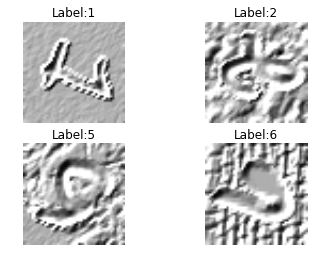
\includegraphics[scale=0.40]{sample_of_images.png}
	\caption{A sampling of the modified MNIST database}
	\label{MNISTSample}
\end{figure}

\section{Methodology}

We used the \href{http://www.numpy.org/}{NumPy package} and the \href{http://www.scikit-learn.org/}{scikit-learn library} to perform feature extraction and selection, implement our classifiers, and analyse our results. 

To implement the advanced Convolution Neural Networks we used the \href{http://pythonhosted.org/nolearn/}{nolearn} package that allows easy layering of neural networks found in \href{http://lasagne.readthedocs.org/}{Lasagne}.

\subsection{Feature Extraction and Preprocessing}


\subsection{Feature Selection}

\subsection{Generating Extra Data}

As per the suggestions of Patrice Simard et al. \cite{Simard} we decided to augment our learners with extra data. The data generated came from two different sources and the effect of the addition of either supplementary dataset is explored later in this paper.

\begin{figure}[h]
	\centering
	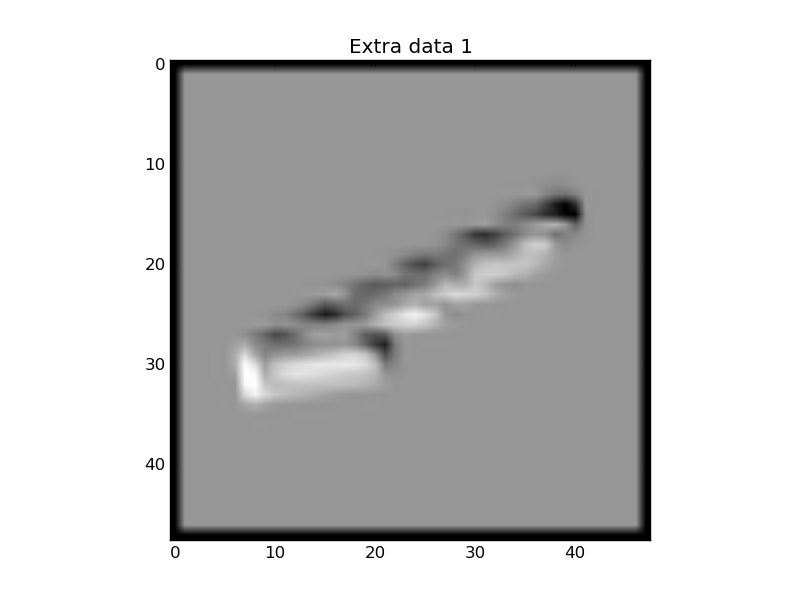
\includegraphics[scale=0.20]{Extradata1.png}
	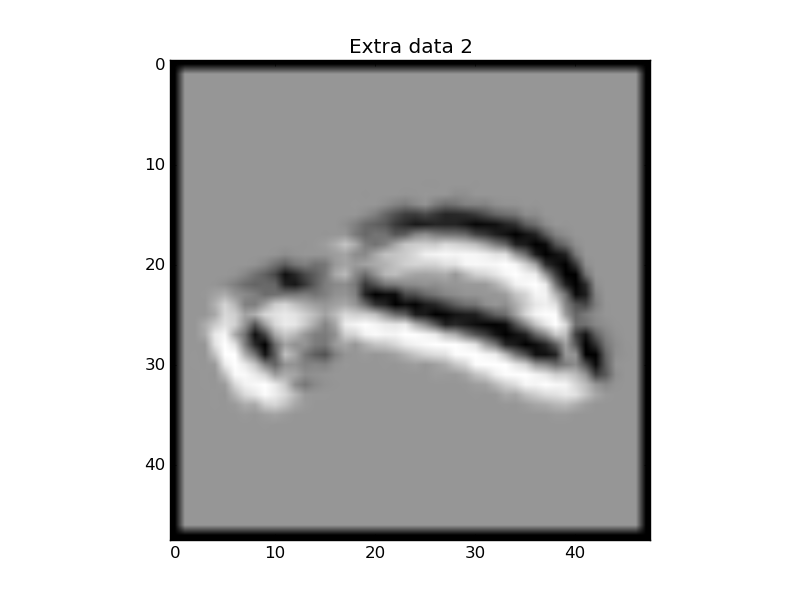
\includegraphics[scale=0.20]{Extradata2.png}
	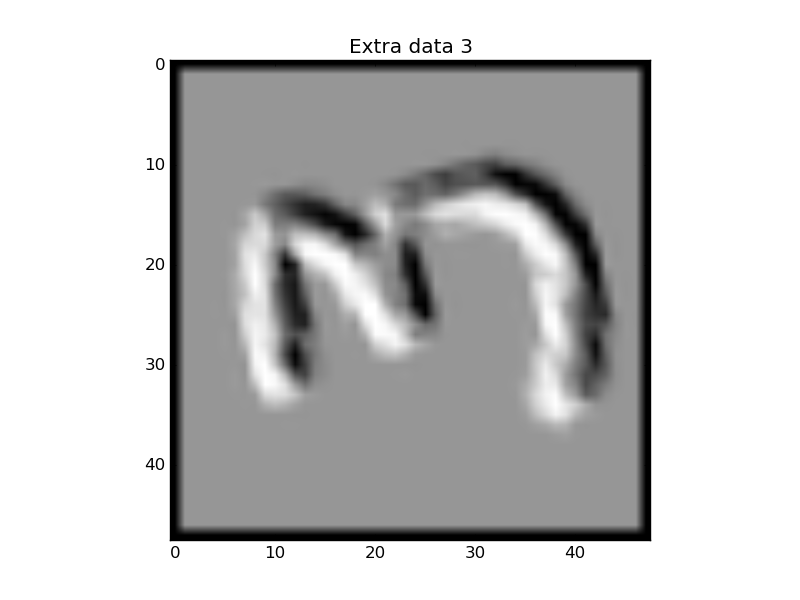
\includegraphics[scale=0.20]{Extradata3.png}
	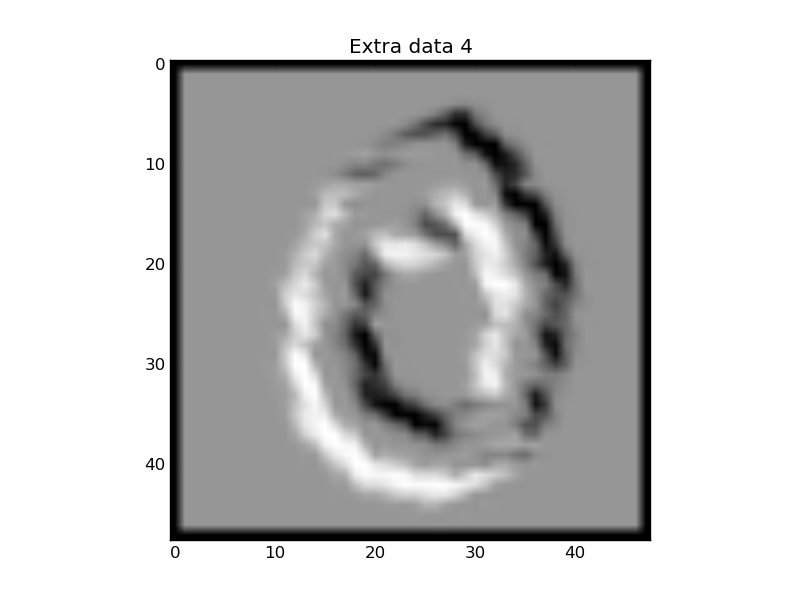
\includegraphics[scale=0.20]{Extradata4.png}
	\caption{Four example image from the "Extra Digits" dataset}
	\label{ExtraData}
\end{figure}

The first additional datasource involved transformations of the original MNIST dataset \cite{MNIST_Original}. We will refer to this dataset as "Extra Digits" throughout the rest of the paper. First we enlarged the images from $28\times 28$ to $48\times 48$. Then we rotated by a random angle $\theta \in  [0,359]$. Finally we applied an emboss to the image. We attempted to add a pattern to the new image as in the modified MNIST dataset, but were unable to find a pattern which we felt maintained the integrity of the image in a way which the patterns used in the modified MNIST dataset did. An example of images from the dataset is shown in \ref{ExtraData}

\begin{figure}[h]
	\centering
	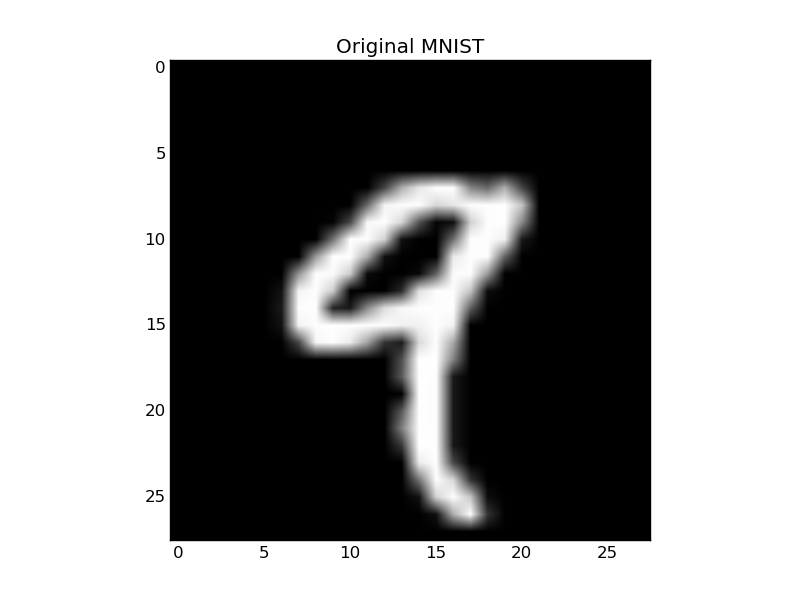
\includegraphics[scale=0.30]{OriginalMNIST.png}
	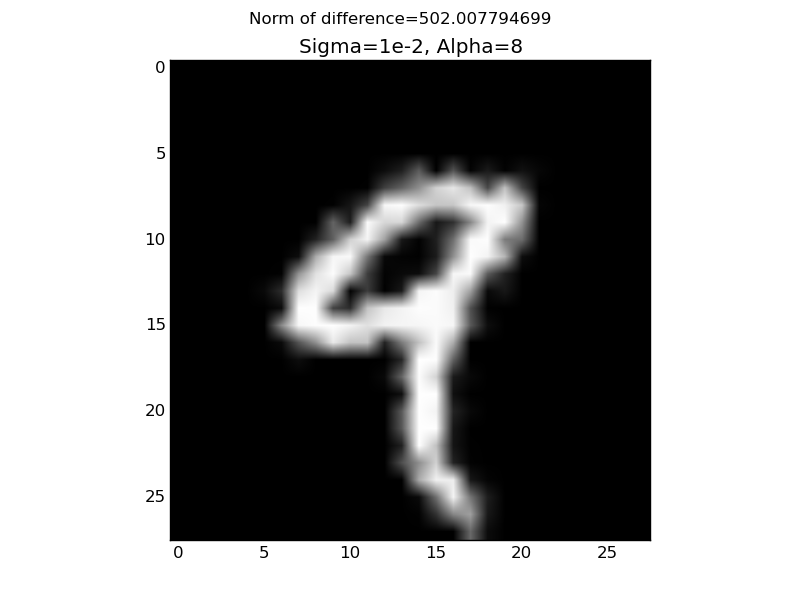
\includegraphics[scale=0.30]{Sigma=1e-2,Alpha=8.png}
	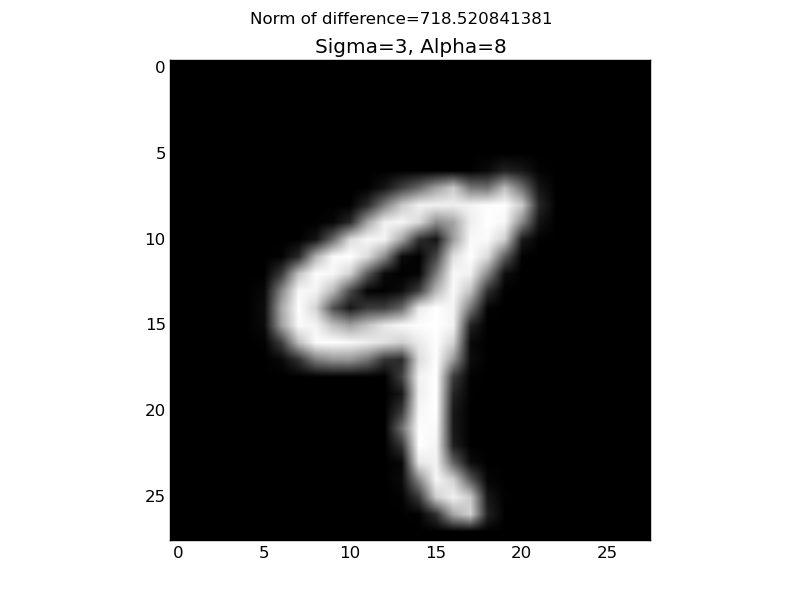
\includegraphics[scale=0.30]{Sigma=3,Alpha=8.png}
	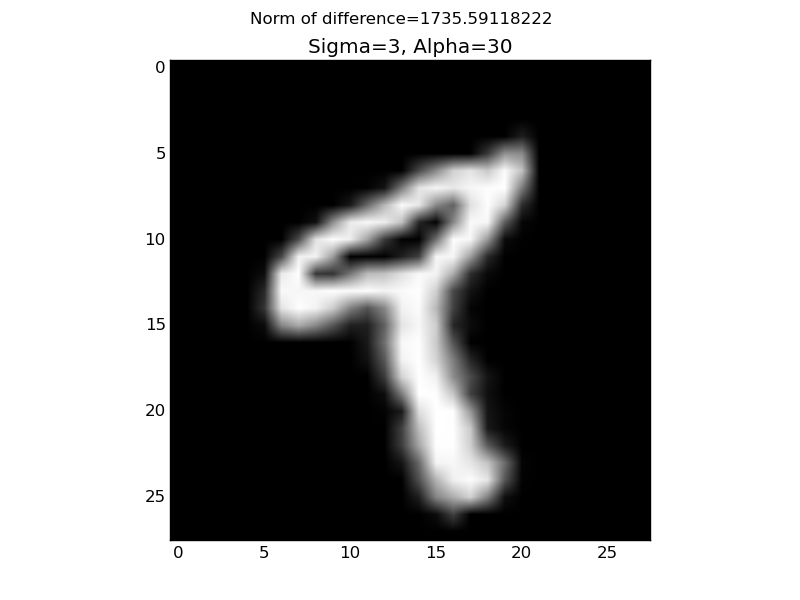
\includegraphics[scale=0.30]{Sigma=3,Alpha=30.png}
	\caption{The effect of varying $\sigma$ and $\alpha$}
	\label{Perturbed}
\end{figure}

The second datasource we attempted to generate was motivated by Patrice Simard et al. \cite{Simard}. This involved performing an affine deformation of the modified MNIST image. We refer to this additional dataset as "Perturbed Modified Digits" throughout the rest of the paper. The methodology for generating these perturbed digits is as follows. Given a $n\times n$ image, we first generate two random $n\times n$ displacement fields $?x(x',y')\rightarrow uniform(-1,1)$ and $?y(x',y')\rightarrow uniform(-1,1)$. We the convolve these displacement fields by a gaussian filter with $\mu = 0$ and $\sigma$ being a variable to the function which defaults to 3. After this we normalize the displacement fields by dividing each element in the field by the norm of the matrix. All the elements in both displacement fields are then multiplied by $\alpha$ which is a variable to the function. We then generate a new $n\times n$ image as such: for each pixel $(i,j)$ in the original, the new value at that pixel is the value at $?x(i,j),?y(i,j)$ in the original picture. Bilinear interpolation is used to determine the value of $new(i,j)=original(?x(i,j),?y(i,j))$ when $?x(i,j),?y(i,j)$ is not an integer. For indices which appear out of bounds of the picture we simply used a default value of 0. \ref{Perturbed} shows the effect of varying $\alpha$ and $\sigma$. The norm of the difference between the original MNIST image and the modified image are included in the pictures.

\begin{figure}[h]
	\centering
	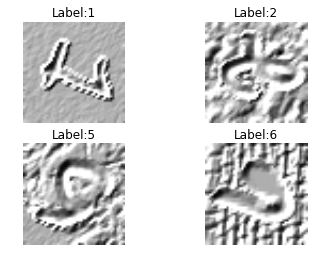
\includegraphics[scale=0.40]{sample_of_images.png}
	\caption{A sampling of the modified MNIST database. It is interesting to notice that the last digit is a 6, even though to the human eye it appears to be a 9.}
	\label{MNISTSample}
\end{figure}

\subsection{Classification Algorithms}

\subsubsection{Baseline: Logistic Regression}
In Logistic Regression, we want to estimate the probability that some random vector $X=(x_1, \ldots, x_n)$ has a class $Y=y_k$, $P(Y=y_k | X=(x_1, \ldots, x_n))$. In the binary case we can derive the following using Bayes rule and conditioning:
\begin{equation*}
\begin{split}
&P(Y=1~|~X) = \frac{P(X, Y=1)}{P(X)}\\
&= \frac{ P(X~|~Y=1)\cdot P(Y=1) }{ P(X~|~Y=1)\cdot P(Y=1) + P(X~|~Y=0)\cdot P(Y=0) }\\
& = \frac{1}{1 + \exp{(-a)}} = \sigma(a) \text{~(Sigmoid Function)}\\
\end{split}
\end{equation*}

where $a=\ln\Big(\frac{P(Y=1~|~X)}{P(Y=0~|~X)}\Big)$ is the log-odds ratio. By approximating the log-odds ratio as a linear decision boundary of the features and weights, $w^T x$ we can use this as an estimate of the class being $Y=1$. We can optimize the Log-likelihood or Cross-Entropy function:

\begin{equation}
	\label{LL}
	L(w) = -\sum_{i=1}^n y_i\log\Big(\sigma(w^Tx_i)\Big) + (1-y_i)\log\Big(1-\sigma(w^Tx_i)\Big)
\end{equation}

and search for the optimal set of weights using the \emph{gradient descent algorithm} with $K$ steps and update rule \ref{LR_update_rule}:

\begin{equation}
\label{LR_update_rule}
	w_{k+1} = w_k + \alpha_k \sum_{i=1}^n \Big( x_i\big(y_i - \sigma(w_k^Tx_i\big) \Big)
\end{equation}

%  @PASCALE PLEASE CHECK THIS?
We did not do any kernel transformations on the data due as this was left to a large margin classifier, the Support Vector Machine found in the next part.

Multi-class classification was implemented using a one-vs-all approach.


\subsubsection{Support Vector Machine}

\subsubsection{Fully Connected Feedforward Neural Network}

\subsubsection{Convolution Neural Network}
The convolution neural network \cite{LeCunn98} is a neural network with specialized layers in which not all neurons are connected to each other. Infact the main component is the subblayer (Fig \ref{convmaxlayer}) which contains the Convolution2D and MaxPool2d pair of layers. A convolution of an image is the result where each pixel is the weighted sum of its neighbouring pixels (moving window weighted sum). This means that our 2D convolution takes a weighted sum of each neighbouring pixel of the handwritten digit. \emph{num\_filters} is the number of moving windows of size \emph{filter\_size} $\times$ \emph{filter\_size} we do convolutions with. In MaxPooling we select the maximum in a region of size \emph{pool\_size} $\times$ \emph{pool\_size} pixels obtained from the 2D convolution.


\begin{figure}[h]
	% \centering
	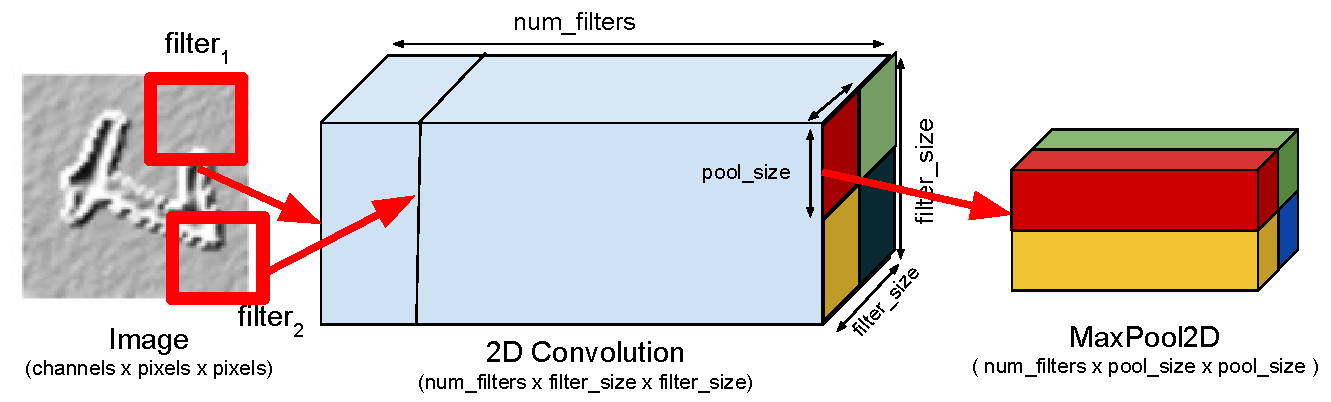
\includegraphics[scale=0.40]{convnet_example.pdf}
	\caption{A simplified example of the sublayer containing Convolution2D layer and a MaxPool2D layer. The variables correspond to the authors implementation of the network. The final network used one,two and three of these sublayers in tandem.}
	\label{convmaxlayer}
\end{figure}

As shown in the (simplified) figure \ref{convmaxlayer}, the convolution conducted on the input is transformed into the 3D spatial arrangement of the filters. This is then subsampled (by selecting the MAX element from each subsection of the filter) to produce the set of outputs that can be reused in future layers. In our architecture we stacked $K$ of the Convolution2D-Maxpool sublayers ($K=\{1,2,3,4\}$) and finally ran the outputs through a fully connected dense layer which had the same number of units as \emph{num\_filters} in the last Convolution2D-Maxpool subplayer. To obtain the final output, we ran this through a $p=0.5$ dropout and then into a fully connected dense layer of size $10$ to make the predictions. This is summarized in Fig \ref{CNNarch}. 

\begin{figure}[h]
	% \centering
	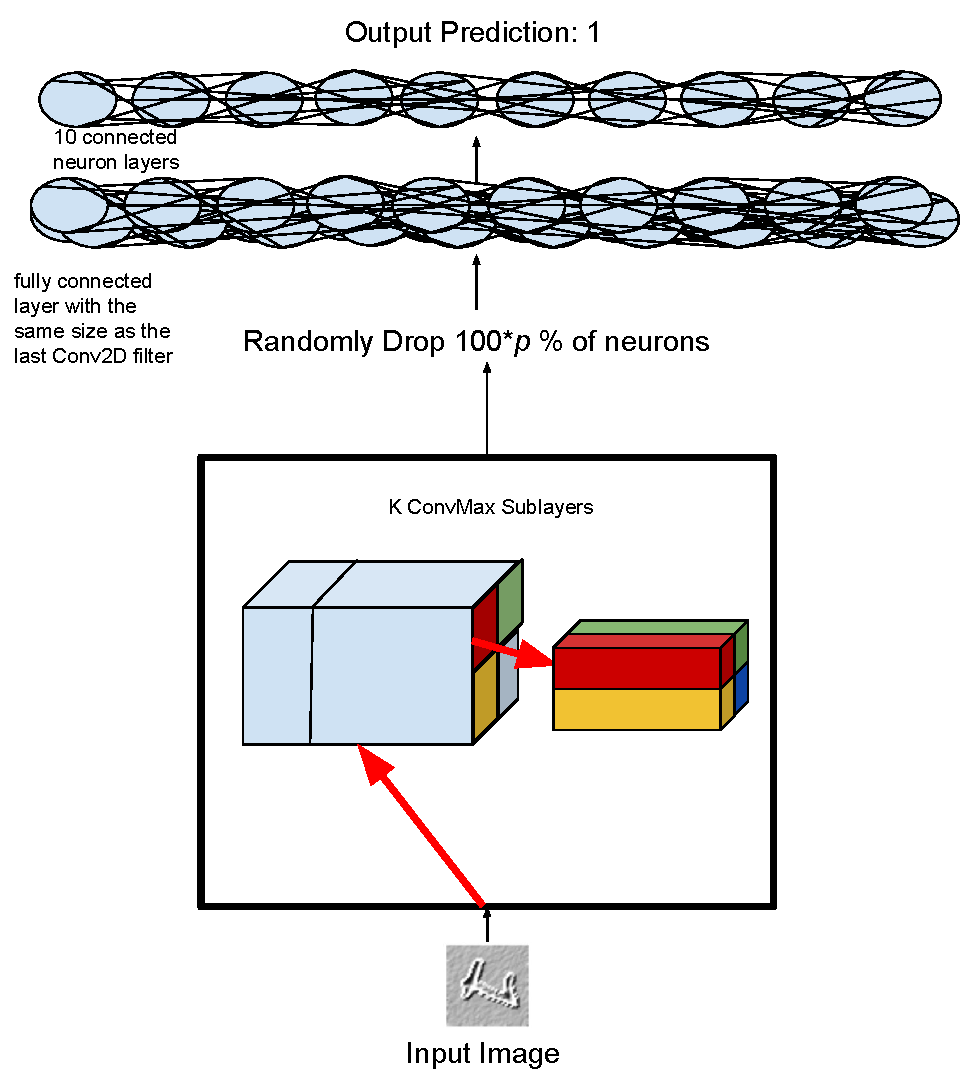
\includegraphics[scale=0.5]{architecture.pdf}
	\caption{The Convolution Neural Architechture included $k$ stacked sublayers shown in Fig \ref{convmaxlayer} connected to a dropout layer and finally fed into a fully connected layer containing $10$ neurons that did the final classification.}
	\label{CNNarch}
\end{figure}

Two methods were used to account for overfitting: (1) dropout\cite{dropout} neurons and (2) addition of extra (perturbed) data. 

In dropout, we randomly delete $50\%$ of the neurons during each forward pass and backpropagation event, this forces neurons to learn a more robust set of features. It is akin to training multiple different networks and this sampling of different neurons during the task reduces the co-dependence of neurons to make predictions. 

Adding perturbed data according to procedure IV-C, ensures that we expose our network to a wider range of possible digits. This means that the network is robust to perturbations in the data and can make better predictions in the event that there are imperfections like distortion, deletions and deformations.

\subsection{Cross-Validation and Choice of Hyperparameters}

\section{Results}

\subsection{Logistic Regression}
The parameters for logistic regression used were the \emph{learning\_rate} ($\alpha$) and \emph{max\_iterations} $K_{\text{steps}}$ that will control how fast we converge to the optimal set of weights for the decision boundary. We used a three-fold cross validation to discover the best parameters, and the results are summarized in Fig \ref{LR_accuracy}. In particular the best combination of parameters are $\alpha=0.01$ and \emph{max\_iterations}=$10000$. Using this we were able to obtain a score of 0.23140 on the Kaggle leaderboard.

\begin{figure}[h]
	\centering
	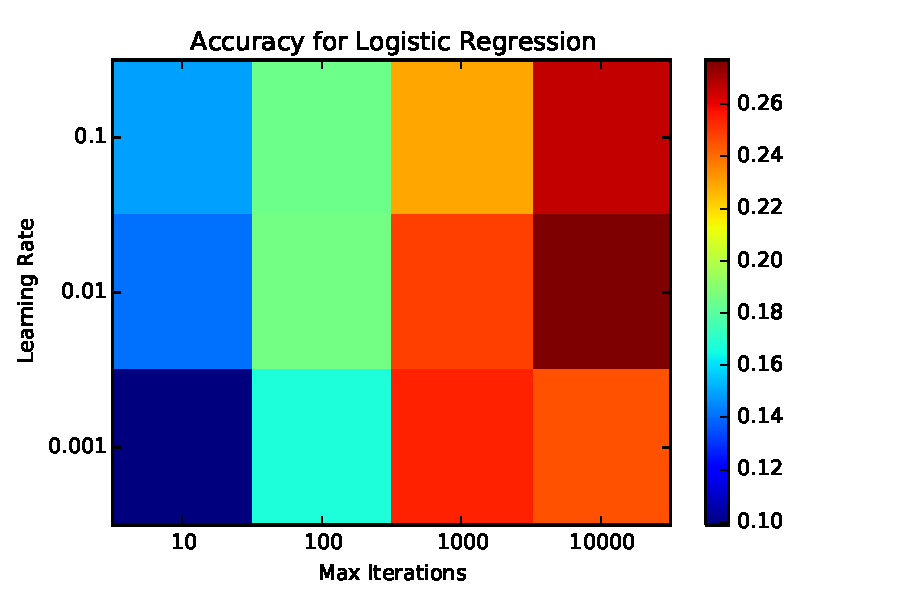
\includegraphics[scale=0.50]{LR_accuracy.pdf}
	\caption{Logistic regression cross validation results, (Red = better accuracy)}
	\label{LR_accuracy}
\end{figure}

\subsection{Feed-forward Neural Network}


\subsection{Convolution Neural Networks}
An epoch is one forward pass and backpropagation event. For a single Convolution-Maxpool layer, we picked the initial number of filters using two-fold cross validation to be $16$ (Fig \ref{CNNacc}). This is because using $16$ filters showed a faster increase in accuracy and selecting a smaller first filter means that there will be fewer parameters to train overall.

After this we trained $2$-CNNs, $3$-CNNs and $4$-CNNs where at each additional Convolution-Maxpool layer we increase the number of filters to extract higher level features. Fig \ref{CNNacc} shows that as the depth of the network increases, we converge to higher accuracy rates.

\begin{figure}[h]
	\centering
	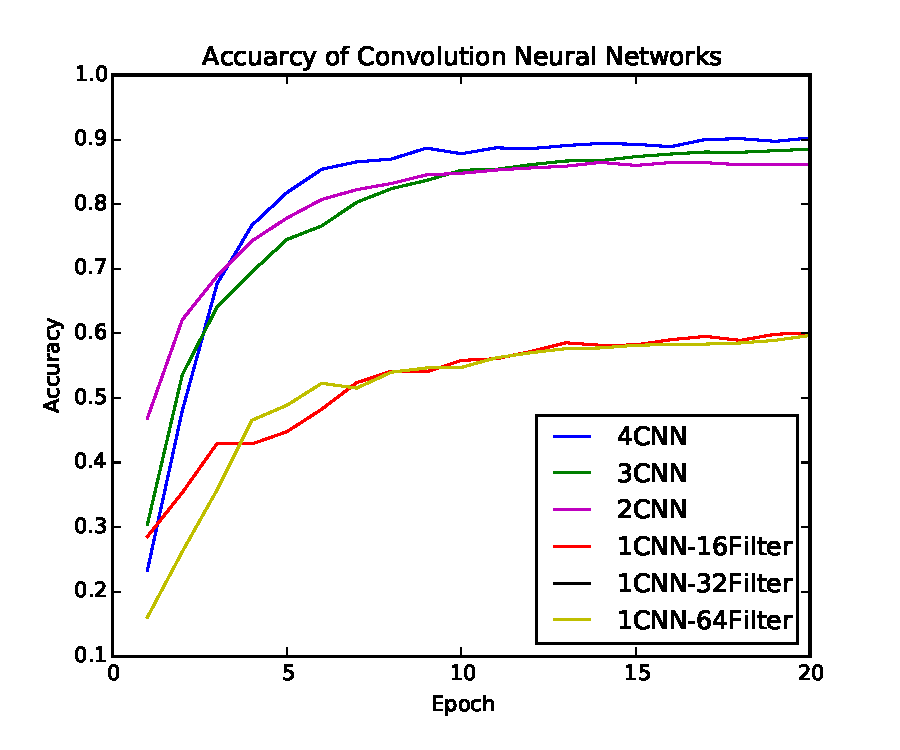
\includegraphics[scale=0.6]{CNNacc.pdf}
	\caption{Accuracy vs Epoch plot}
	\label{CNNacc}
\end{figure}

Further examination on the $4$-CNN shows that (without extra data) we converge to our optimal set of weights after $10-12$ epochs (Fig \ref{C4NNacc}. This prediction scored 0.90940 on the Kaggle leaderboard.

\begin{figure}[h]
	\centering
	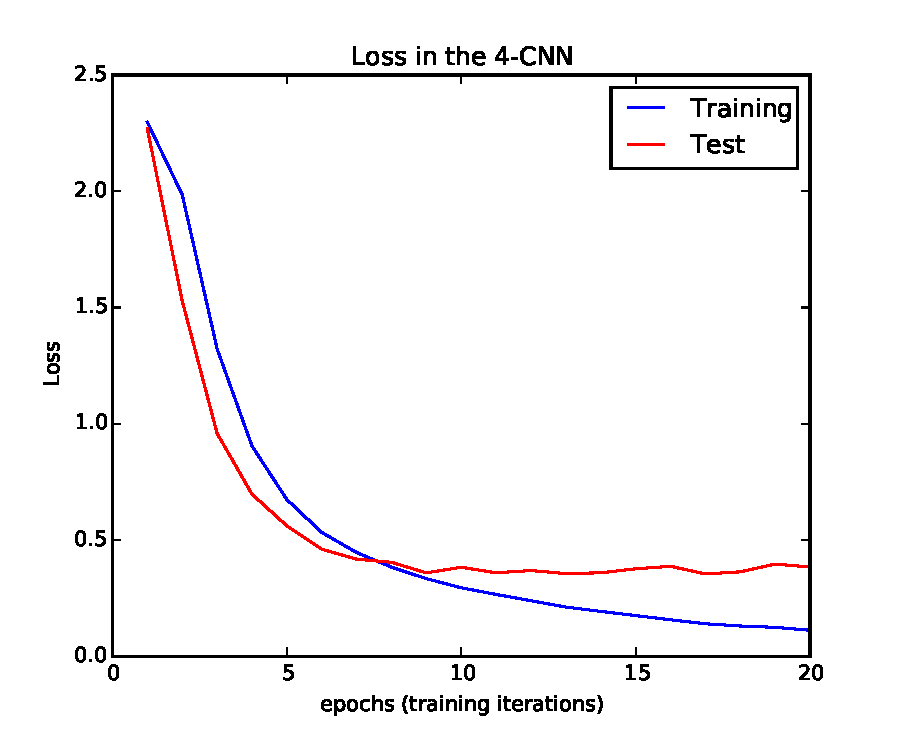
\includegraphics[scale=0.6]{4CNNloss.pdf}
	\caption{Loss in the 4CNN (without extra data)}
	\label{C4NNacc}
\end{figure}

As a final attempt to boost our accuracy rates, we artificially inflated the dataset to include $50,000$ more images randomly perturbed bringing the total dataset size to $100,000$. We can compare how this classifier performs against the other $4$-CNNs in Fig \ref{CNNacc} and how quickly it converges to a solution in Fig \ref{C4NNacc}. The classifier trained with extra data scored 0.XXX on the Kaggle leaderboard effectively putting the classifier in the top $25\%$ of classifiers for this project.


\section{Discussion}


\subsection{Feature Extraction and Selection}



\subsection{Classifier Performance}

\begin{figure}[h]
	\centering
	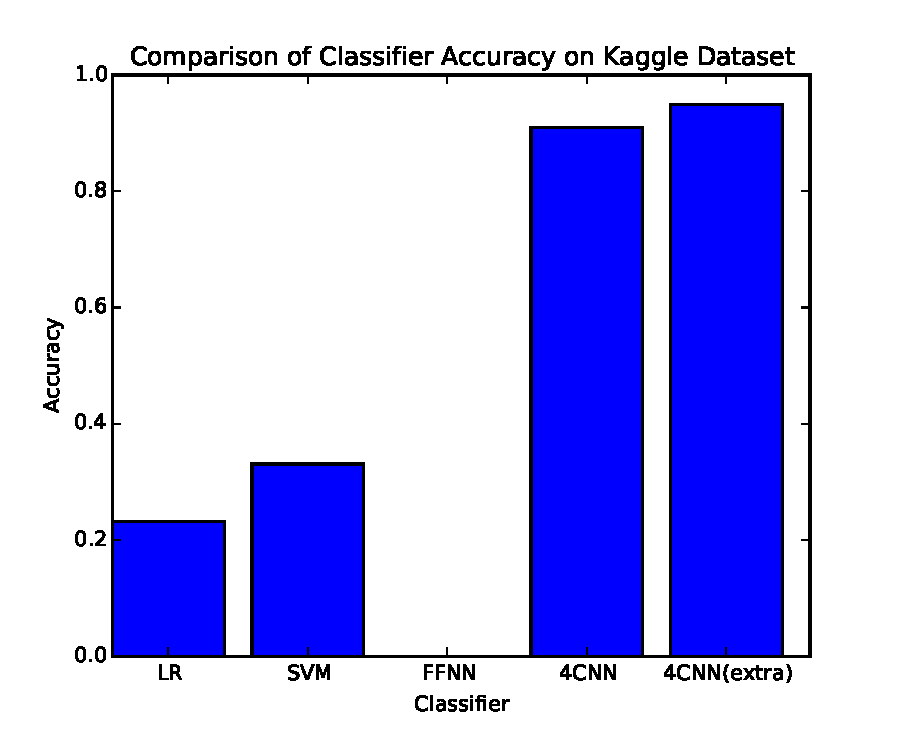
\includegraphics[scale=0.6]{cross-classifier-acc.pdf}
	\caption{Cross-classifier accuracy showing the accuracy of each classifier on a validation set}
	\label{crossacc}
\end{figure}


\subsection{Future Work}
Next steps involve investigation into a Spatial Transformer Network \cite{STN} and see how it compares to the industry standard Convolution Neural Network used in this paper.


\section{Statement of Contributions}

\begin{enumerate}
\item D.R.
\item Z.A. wrote the Logistic Regression classifier from scratch. Z.A. also developed the Convolution Neural Network Architecture and ran experiments to cross validate different layering approaches.
\item P.G.
\item All authors contributed equally to the generation of this report, including graphics.
\end{enumerate}


\section{Integrity of work}
We hereby state that all the work presented in this report is that of the authors.
\begin{thebibliography}{9}

\bibitem{MNIST_Original}
LeCun Y., Cortes, C. and Burges C.J.C.
	\emph{The MNIST Database of handwritten digits}
	http://yann.lecun.com/exdb/mnist/
% inspiration for graphic http://cs231n.github.io/convolutional-networks/


\bibitem{LeCunn98}
Lecun Y., Bengio Y., and Haffner P.
 \emph{Gradient-Based Learning Applied to Document Recognition}
 Proceedings of the IEEE,
 1998.

% \bibitem{MNIST_Original}
% Lecun Y., Cortes C. Burges C.
% \emph{The MNIST database of handwritten digits} 
 
\bibitem{ML_textcat}
 Sebastini, F.
  \emph{Machine Learning in Automated Text Categorization}
  ACM Computing Surveys (CSUR) 34
  2002.

\bibitem{CNN_committees}
 Claudiu D. and Meier U. et al.
  \emph{Convolutional Neural Network Committees For Handwritten Character
Classification}
  ACM Computing Surveys (CSUR) 34
  2002.

\bibitem{STN}
 Jaderberg, M., et al.
  \emph{Spatial Transformer Networks}
  ArXiv
  2015
  
\bibitem{Simard}
  Simard F., Steinkraus D., Platt J.
  \emph{Best Practices for Convolutional Neural Networks
Applied to Visual Document Analysis}
	Microsoft
    http://research.microsoft.com/pubs/68920/icdar03.pdf.


\bibitem{dropout}
Krizhevsky A., Sutskever I., and Hinton G.E.
\emph{ImageNet Classification with Deep Convolution Neural Networks}
	NIPS 2012

\end{thebibliography}

\end{document}
